\documentclass[a4paper,12pt]{article}
\usepackage[utf8]{inputenc}
\usepackage{fancyhdr}
\usepackage{graphicx}
\usepackage{lastpage}
\usepackage[parfill]{parskip}
\usepackage{xcolor}
\usepackage{geometry}
\usepackage{algorithm}
\usepackage{algpseudocode}

\makeatletter
\renewcommand{\ALG@beginalgorithmic}{\scriptsize}
\makeatother

\graphicspath{ {./report_images/} }


\fancypagestyle{style1}{
\lhead{Control \#1924744}
\rhead{Page \thepage \hspace{1pt} of \pageref{LastPage}}
\cfoot{}
}

\fancypagestyle{style2}{
\lhead{Control \#1924744}
\rhead{Page \thepage \hspace{1pt}}
\cfoot{}
}




\begin{document}

\title{Developing an Aerial Disaster \\* Relief Response System}
\author{Control \#1924744}
\date{28th January 2019}
\maketitle
\newpage


\pagenumbering{roman}
\pagestyle{style2}

\section*{\hfil Summary\hfil}
\begin{center}
\textit{"All models are wrong but some are useful''} \\*
\end{center}
As asked by HELP. INC, we devised a drone disaster response system to deal with future disasters in Puerto Rico.
Our model relied on first determining where to place the containers and then applying our own algorithm to efficiently pack containers known as the Cuboid Reduction Method (CRM).
In order to determine how many containers to place we plotted the range of each drone from a medical centre. We then triangulated the regions to where containers could be placed.
Using this technique we found that a minimum of 3 containers were required to supply all the medical centres.

Our algorithm known as the CRM splits the container into a finite number of cuboids of equal dimensions, which we use for packing separate supplies.
We then used the medical package ratio of each medical centre to calculate how many cuboids should be allocated to each type of medical package.
\\*In order to determine how many containers to place we plotted the range of each drone from a medical centre and triangulated the regions to find where containers could be placed.
Using this technique we found that a minimum of 3 containers were required to supply all the medical centres. \\*\\*
After finding out where to place containers and which medical centres they would supply, we found the ratio of medical packages to pack in each container.
The CRM was then used to calculate how many days each container's supplies could last and how much of each medical package had to be packed in.
\\*
In order to perform our second objective of mapping roads we approximated the major roads between each medical centre using a series of straight lines.
We managed to approximate our roads to an accuracy of up to 96\% and plotted a map of how far a recon drone could travel done each road.\\* We determined that up to 100\% of the road network between medical centres
could be mapped if we allocated an additional two drones to our two furthest containers to go as far as possible without returning. Otherwise up to 60\% of the road network is mappable.

Using data obtained for the 2017 Puerto Rico crisis we found that our strategy would more than sufficiently deal with the problem of supplying medical centres and mapping roads. This leads us to be confident in the
power of using a DroneGo fleet model to deal with future disasters in Puerto Rico or similar environments.

\newpage

\section*{\hfil MEMO\hfil}
\hrulefill

\bf{Date:} \normalfont{28th January 2019}\\*\\*
\bf{To:} \normalfont{Ms. Smith (CEO)}\\*\\*
\bf{From:} \normalfont{\#1924744}\\*\\*
\bf{Subject:} \normalfont{Puerto Rico Disaster Model}\\*\\*
{\color{black}\hrule}
In this memorandum, we present to you our model of a drone based disaster response system capable of dealing with the Puerto Rico hurricane scenario. After careful consideration of the demands of the situation, we have selected a suitable fleet of drones and set of medical package configurations that may be employed in response to such an emergency. Below, we outline the main components of our model and summarize the results of its performance.

Our first challenge was determining the ideal packing configurations for ISO containers. We treated this as an optimization problem. Through doing so, we were able to devise three different algorithms (In-Fitter, Cuboid Reduction Method and RatioCheck) that we used in together to figure out how to pack supplies in the most efficient way possible. Our model demanded the use of three ISO containers to supply our medical centres.

To select the drones suitable for delivery we prioritized their maximum range over the delivery time. We concluded that given a 24 hour delivery deadline, speed was a less important factor. Using algorithms, we concluded that we would be able to supply our medical centres adequately. The time frames generated ranged from 8 months for a container supplying several medical centres to 8 years for one medical centre. Furthermore, this strategy allowed us to map roughly 60% of the major road networks linking the medical centres.

While this model is not perfect, when compared to data from the 2017 Puerto Rico hurricane scenario, it is evident that the time frame of support provided is certainly sufficient for most medical centres. Therefore, we conclude that while one must initially invest more costs in allocating three ISO containers to the disaster area, the corresponding payoff largely merits the price. We use this as justification to present our design recommendations to you in the report that follows.

\newpage


\tableofcontents
\newpage



\newpage

\pagenumbering{arabic}
\pagestyle{style1}


\section{Introduction}

\subsection{Background}
Puerto Rico is a small US territory situated on the 18th parallel. It has a population of approx 3.29 mill and a population density focused around the coast,
with San Juan being its most populated area$^{1}$. Puerto Rico's tropical climate is starkly divided between the northern two thirds and southern third of the island.
The northern side experiences much more humid weather than the southern side and is the area we are most concerned with.\\* Puerto Rico's annual rainfall also differs greatly between the eastern front, where the Sierra de Luquillo rainforest is located and the western side of the island.
May to November is generally considered to be hurricane season in Puerto Rico while December to March is known as the dry season$^{2}$.
In recent years climate change has caused an acceleration of storms in the tropical belt and poses a serious threat to the future prosperity of Puerto Rico. Efforts are ongoing to combat this problem but critics have been outspoken against the lack
of focused effort to deal with it more$^{3}$.

\begin{figure}[h]
\centering
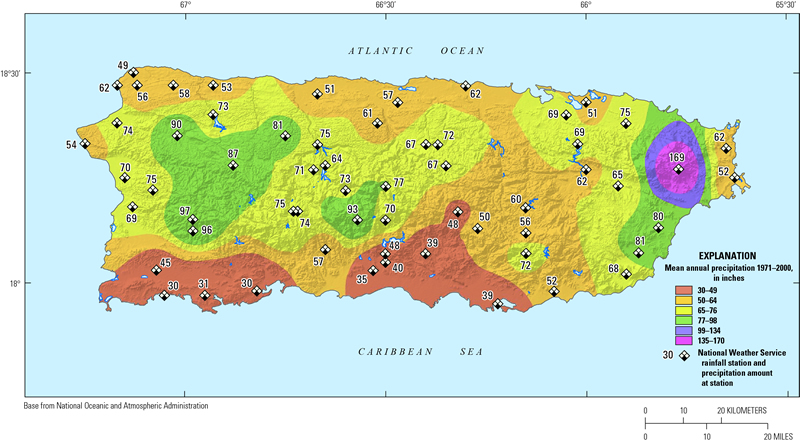
\includegraphics[scale =0.5]{Rainfall}
\caption{Mean Annual Precipitation 1971-2000}
\label{rainfall}
\end{figure}

Hurricane Maria struck Puerto Rico on September 16th 2017 and destroyed Puerto Rico's electrical and communication grid. With over 2900 fatalities it quickly became
the worst natural disaster to ever hit Puerto Rico.$^4$

\subsection{Problem Restatement}
As asked by HELP.INC, we were tasked with developing a DroneGo drone fleet that could help deal with future disasters in
Puerto Rico by analyzing the 2017 hurricane. Our task is divided into two main objectives;
\begin{itemize}
\item[-]Delivering required medical packages to the associated medical centres each day.
\item[-]Assessing the major highways and roads that link these centres for ground route planning
\end{itemize}
In order to achieve our first objective we decided to start from the bottom and make our way up. That is to say, we began by seeing how to fit medical packages into cargo bay containers, following this
we moved onto seeing which CB-MP (cargo bay to medical package) combination would suit each medical centre's daily needs. Moving up the ladder we ranked our drones by maximum range and so forth and so on.
\\*One major problem appeared to be where to leave a container and how to pack items into a container, we recognized the latter as an optimization problem, specifically a 'bin packing problem'$^5$.

\section{Terminology}
Throughout the paper acronyms and numbers may be used to abbreviate repeated words and terms. While these are usually explained elsewhere they can also be found here for convenience.

\begin{center}
\begin{tabular}{ |c|l| }
\hline
 \bf{Acronym} & \bf{Explanation}  \\\hline
 CB & Drone Cargo Bay \\
 MP or M & Medical Package \\
 MC & Medical Centre\\
 C & Container \\
 FOV & Field of View \\
 \hline
\end{tabular}
\end{center}
The following medical centres were also represented using numbers in the maps found in subsequent sections.

\begin{center}
\begin{tabular}{ |c|l| }
 \hline
 Number & Medical Centre  \\\hline
 1 & Caribbean Medical Centre, Fajardo \\
 2 & Hospital HIMA, San Pablo \\
 3 & Hospital Pavia Santurce, San Juan \\
 4 & Puerto Rico Children's Hospital, Bayamon \\
 5 & Hospital Pavia Arecibo, Arecibo  \\
 \hline
\end{tabular}
\end{center}

\section{The Assumptions}
The following core assumptions were made before starting our first model. These were necessary to fully understand the strategy we would
need to develop to distribute medical supplies and survey roads:

\begin{itemize}
\item[-]Each drone must return to a container after completing one or more deliveries.
        This is because we assume drones must be recharged/restocked before setting out again.
\item[-]Drones can only be used once a day. Drone LiPo batteries are some of the slowest charging batteries around$^{6}$ and
        the size of the drone suggests recharging will take an entire day.
\item[-]Drones could not be recharged at medical centres.
        Initially we considered charging them in the centres but after research, discovered that
        many hospitals in the 2017 crisis were without power or generator fuel.
\item[-]The contents of every container will not be damaged or suffer from any accidental malfunction.
\item[-]Major roads and highways can be approximated as straight lines or a zigzag of lines when needed. This is justified as small road deviations will only be slightly longer than straight lines.
\item[-]Drones are given special permission to fly in airport airspace. This is because drone delivery in San Juan would be impossible as drones would have to break FAA regulations$^7$.
\item[-]Drones are assumed to be unable to glide without power. If drones could glide then only one container would be theoretically necessary however this is too unlikely.
\item[-]Items are packed into the container in such a way that removing the necessary items will not cause issues or delays.
\item[-]The drone's CB is included in the drone's container dimensions.
\end{itemize}

\section{The Ideal Setup}

In order to understand which drone was suitable to use in deliveries it was necessary to begin with the core fundamentals
of how a cargo bay would store medical packages. This was noticed to be a bin packing problem however we focused solely on packing MP1s into both CBs.

\subsection{Algorithm 1: In-fitter Algorithm}
We developed our own algorithm known as the 'In-fitter' algorithm that would determine the best packing configuration of one type of MP into a container.

\begin{algorithm}
  \caption{'In-fitter' Algorithm }
  \label{array-sum}
  \begin{algorithmic}[1]
    \Procedure{infitter}{$box\textsubscript{1}$, $box\textsubscript{2}$}
    \State $ParameterOne$: $box\textsubscript{1}$ Dimensions of the bigger box (Array) $[L, W, H]$
    \State $ParameterTwo$: $box\textsubscript{1}$ Dimensions of the smaller box (Array) $[L, W, H]$
    \State $Output$: The most amount of $box\textsubscript{2}$'s that will fit into $box\textsubscript{1}$
    \State
    \State $perms \leftarrow [1,2,3;1,3,2;2,1,3;2,3,1;3,1,2;3,2,1]$
    \Comment{permutations of box orientation}
    \State $amountFit \leftarrow [6] $
    \For {$i = 1$ to $6$ }
    \State $boxL \leftarrow box\textsubscript{2}[perms[i][1]] $ \Comment{get current permutation configuration}
    \State $boxW \leftarrow box\textsubscript{2}[perms[i][2]] $
    \State $boxH \leftarrow box\textsubscript{2}[perms[i][3]] $
    \State
    \State $amountL \leftarrow floor( box\textsubscript{1}[1]/boxL )$
    \State $amountW \leftarrow floor( box\textsubscript{1}[2]/boxW )$
    \State $amountH \leftarrow floor( box\textsubscript{1}[3]/boxH )$
    \State $amountFit[i] \leftarrow (amountL * amountW * amountH)$
    \EndFor
    \State Return $findLargest(amountFit)$
    \EndProcedure
  \end{algorithmic}
\end{algorithm}


\subsection{P-CB (Package to Cargo Bay) Configuration}
Since $MP_2$ and $MP_3$ can each fit once inside $MP_1$ \bf{we can set a lowest bound} \normalfont{to how many MPs can be stored in each CB.}\\*
Using the INFITTER algorithm we saw that 2 $MP_1$ can be held inside a CB1 and 12 $MP_1$ inside a CB2.  The table below illustrates this further:

\begin{center}
\begin{tabular}{ |c|c| }
 \hline
 Cargo Bay & Smallest Possible Linear Combination of $MP_1, MP_2$ and $MP_3$\\\hline
 1 & $aMP_1 + bMP_2 = 2$  \\
 2 & $aMP_1 + bMP_2 + cMP_3 = 12$ \\
 \hline
\end{tabular}
\end{center}

As seen in the table, CB1 is limited to only sending combinations of $MP_1$ and $MP_2$, while CB2 can have combinations of all three.

\subsection{CB Combinations For Medical Centres}
Here we look at how many deliveries would be required to each medical centre depending on the drone cargo bay type.
\begin{center}
\begin{tabular}{ |c|c|c|c| }
 \hline
 MC & Daily Need & CB1 & CB2 \\\hline
  1 & $(M_1,M_3)$ & $(M_1,M_3)$ & $(M_1,M_3)$  \\
  2 & $(M_1,M_1,M_3)$ & $(M_1),(M_1,M_3)$ & $(M_1,M_1,M_3)$  \\
  3 & $(M_1,M_2)$ & $(M_1,M_2)$ & $ (M_1,M_2)$  \\
  4 & $(M_1,M_1,M_2,M_3,M_3)$ & $(M_1,M_2),(M_1,M_3),(M_3)$ & $(M_1,M_1,M_2,M_3,M_3)$  \\
  5 & $(M_1)$ & $(M_1)$ & $(M_1)$  \\
\hline
\end{tabular}
\end{center}
Looking at the table we can see that 3 and 5 both have available CB's that match their daily needs (CB1 and CB2 respectively).
For the others, it is harder to immediately see which configuration will suit them.\\*
It is now important to determine a strategy by which these MP's will be delivered to each location.

\section{Containers and Locations}
\subsection{Eliminating Unnecessary Drones}
Looking at the requirements of each medical centre it is obvious that the most important factor is the range a drone can travel rather than the speed.
This is because a drone that arrives 40 mins earlier is trivial when operating on a 24hr deadline for delivery.
We then proceeded to rank drones in terms of their distance as well as if they were a CB1 or CB2 type drone.
Drones A and H were immediately discarded as they were either completely useless for the task required or simply very inefficient.

\begin{center}
\begin{tabular}{ |c|c|c| }
 \hline
 Drone & Distance (Km) & CB \\\hline
  B & 24.4 & 1 \\
  C & 17.1 & 2  \\
  D & 7.9 & 1 \\
  E & 6.5 & 2 \\
  F & 14.4 & 2 \\
  G & 7.5 & 2 \\
 \hline
\end{tabular}
\end{center}
Looking at the table we can see that the best CB1 drone is drone B, likewise the best CB2 drone is drone C. At second place are drones D and F respectively.

\subsection{Drone Flight Radius}
Before developing a configuration for each container it was important to see where containers could be placed regardless of their contents.
Using simple geometry and a generated map of Puerto Rico we could instantly visualize the radial distance a drone could travel from a medical centre.\\*
The region that intercepted each circle would tell us where we could place a container. This allowed us to immediately discard any unsuitable area and focus on where the circle boundaries overlapped.
\\*We also imposed a few local assumptions to realistically reflect each drone's performance.

\begin{itemize}
\item[-]Drones would have a 5 percent range reduction due to carrying a large payload.
\item[-]Drones would have an additional range reduction from time used climbing to 400 feet (121m) and descending back down. 400 feet is the FAA drone height limit.$^7$
\end{itemize}

\begin{figure}[h]
\centering
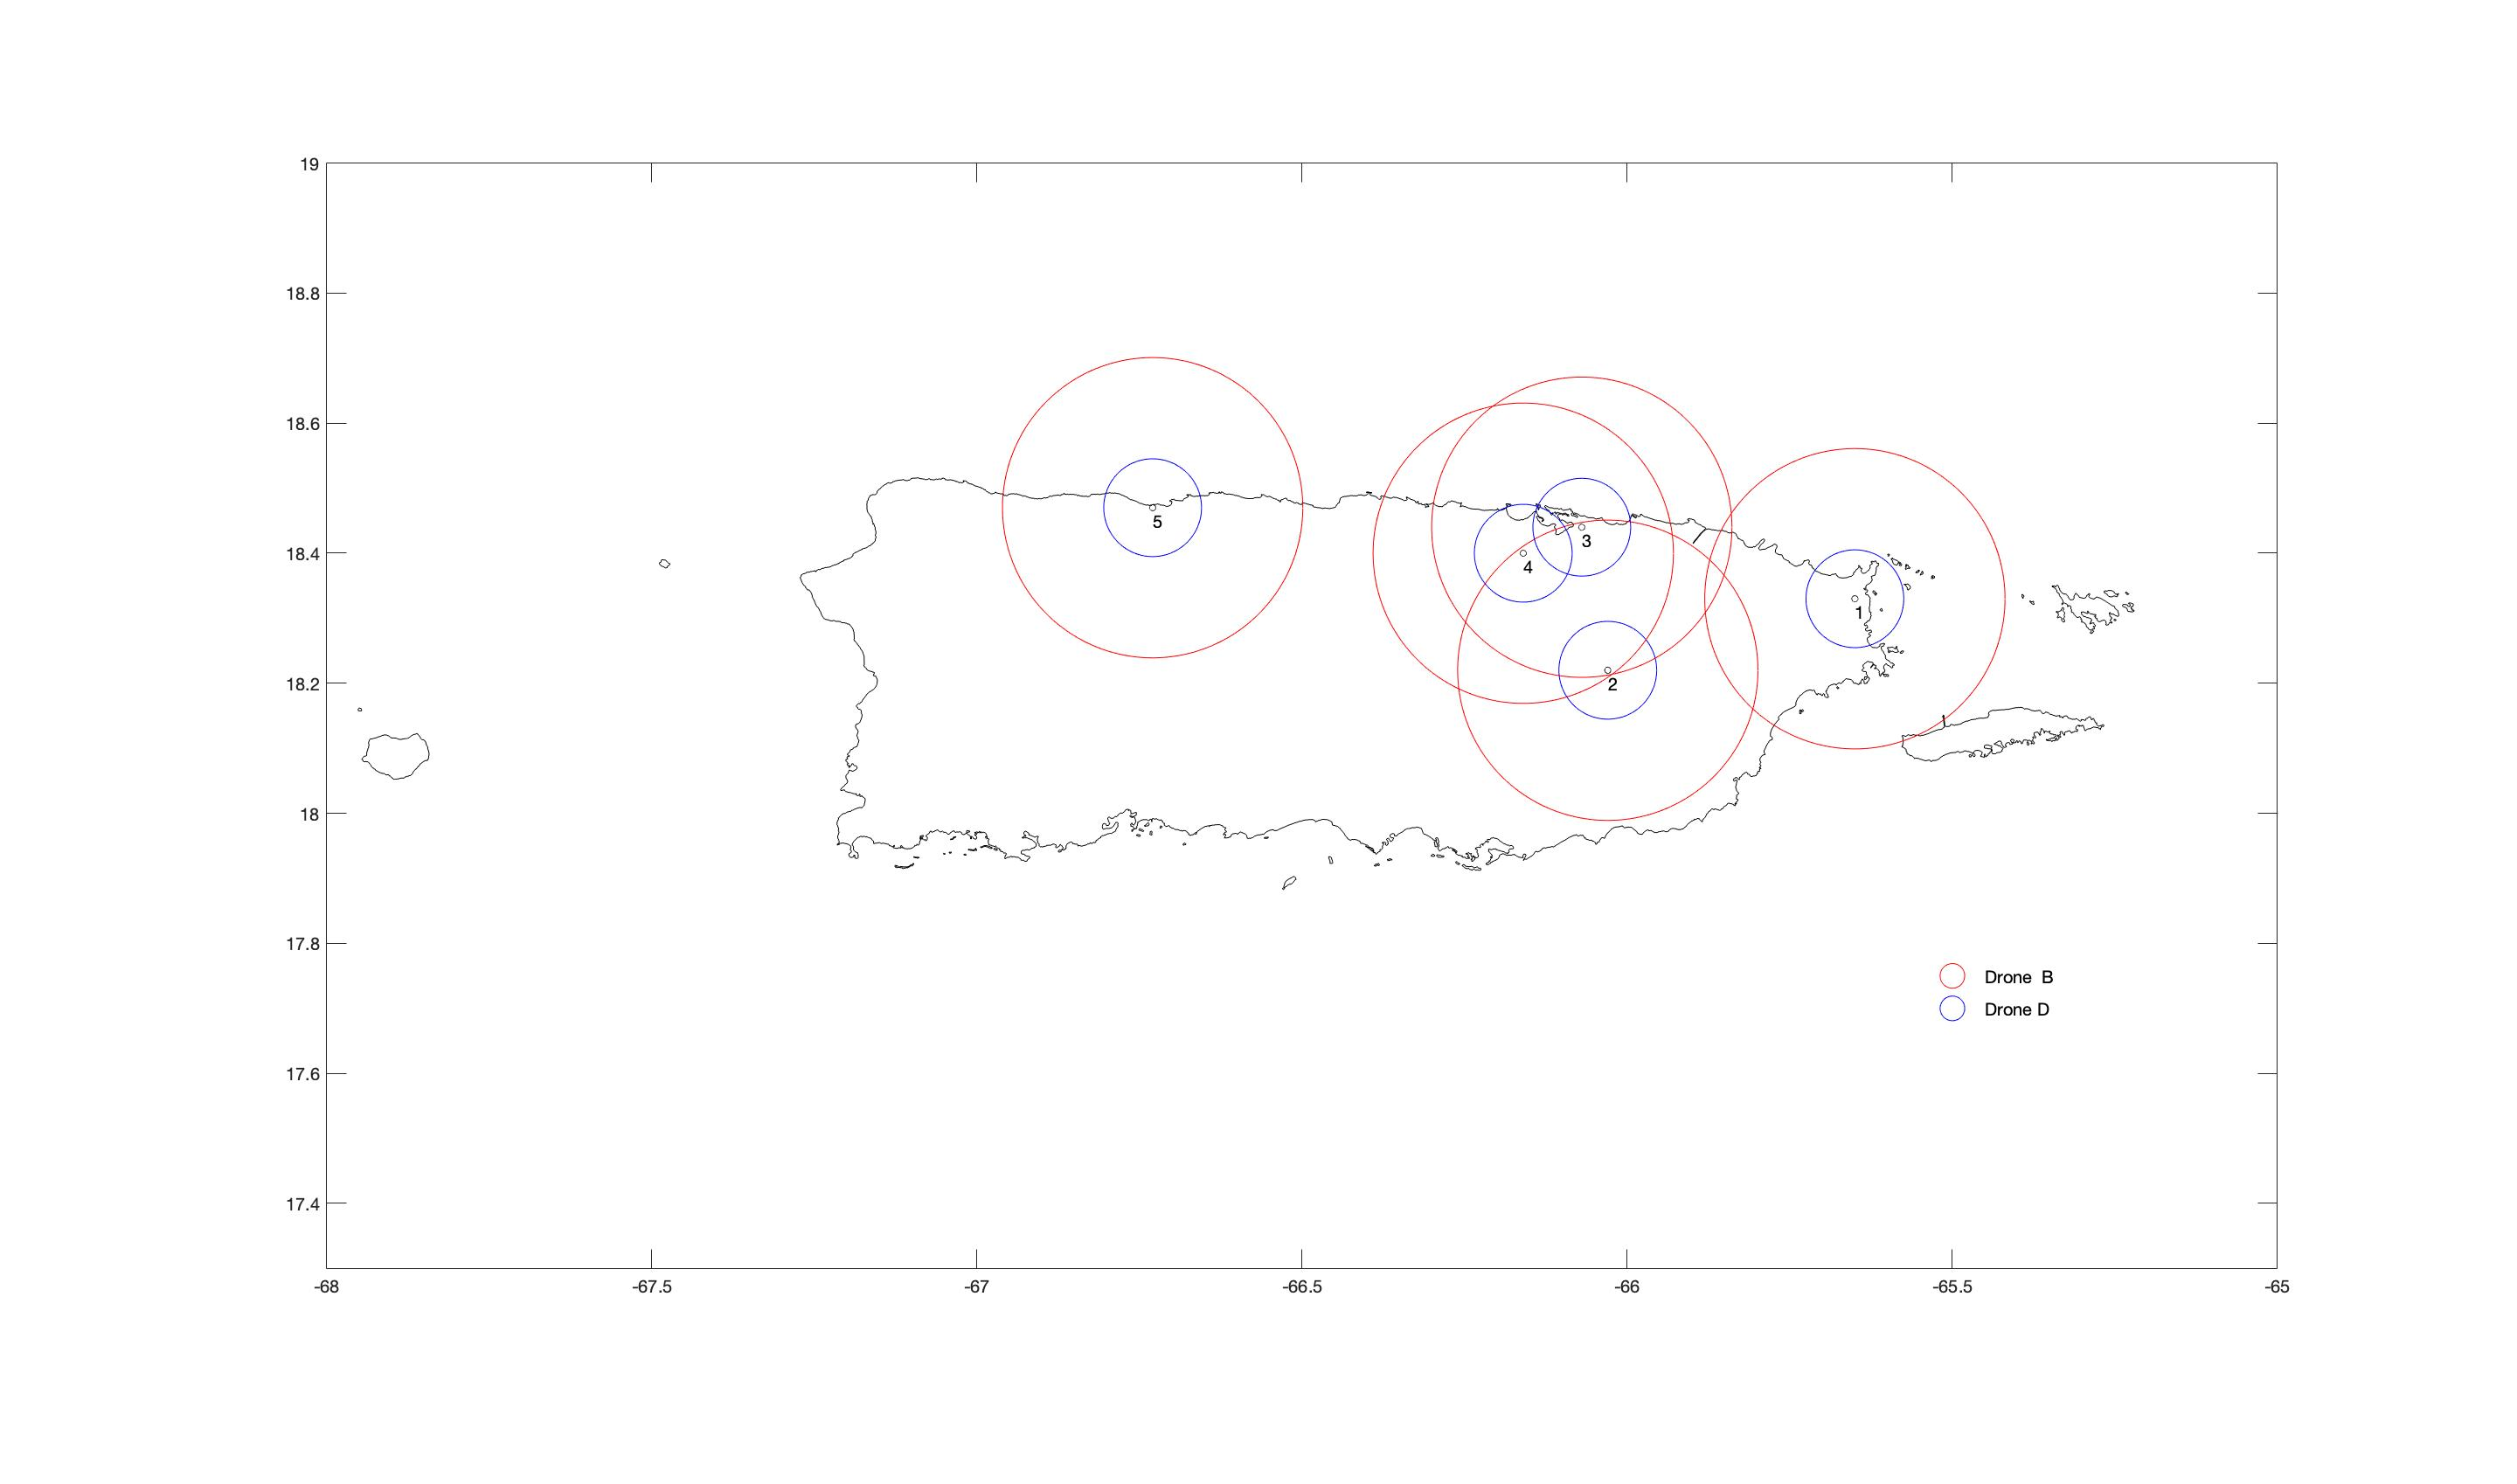
\includegraphics[scale =0.15]{CB1}
\caption{CB1 drone radii around each MC}
\label{cb1}
\end{figure}

\begin{figure}[h]
\centering
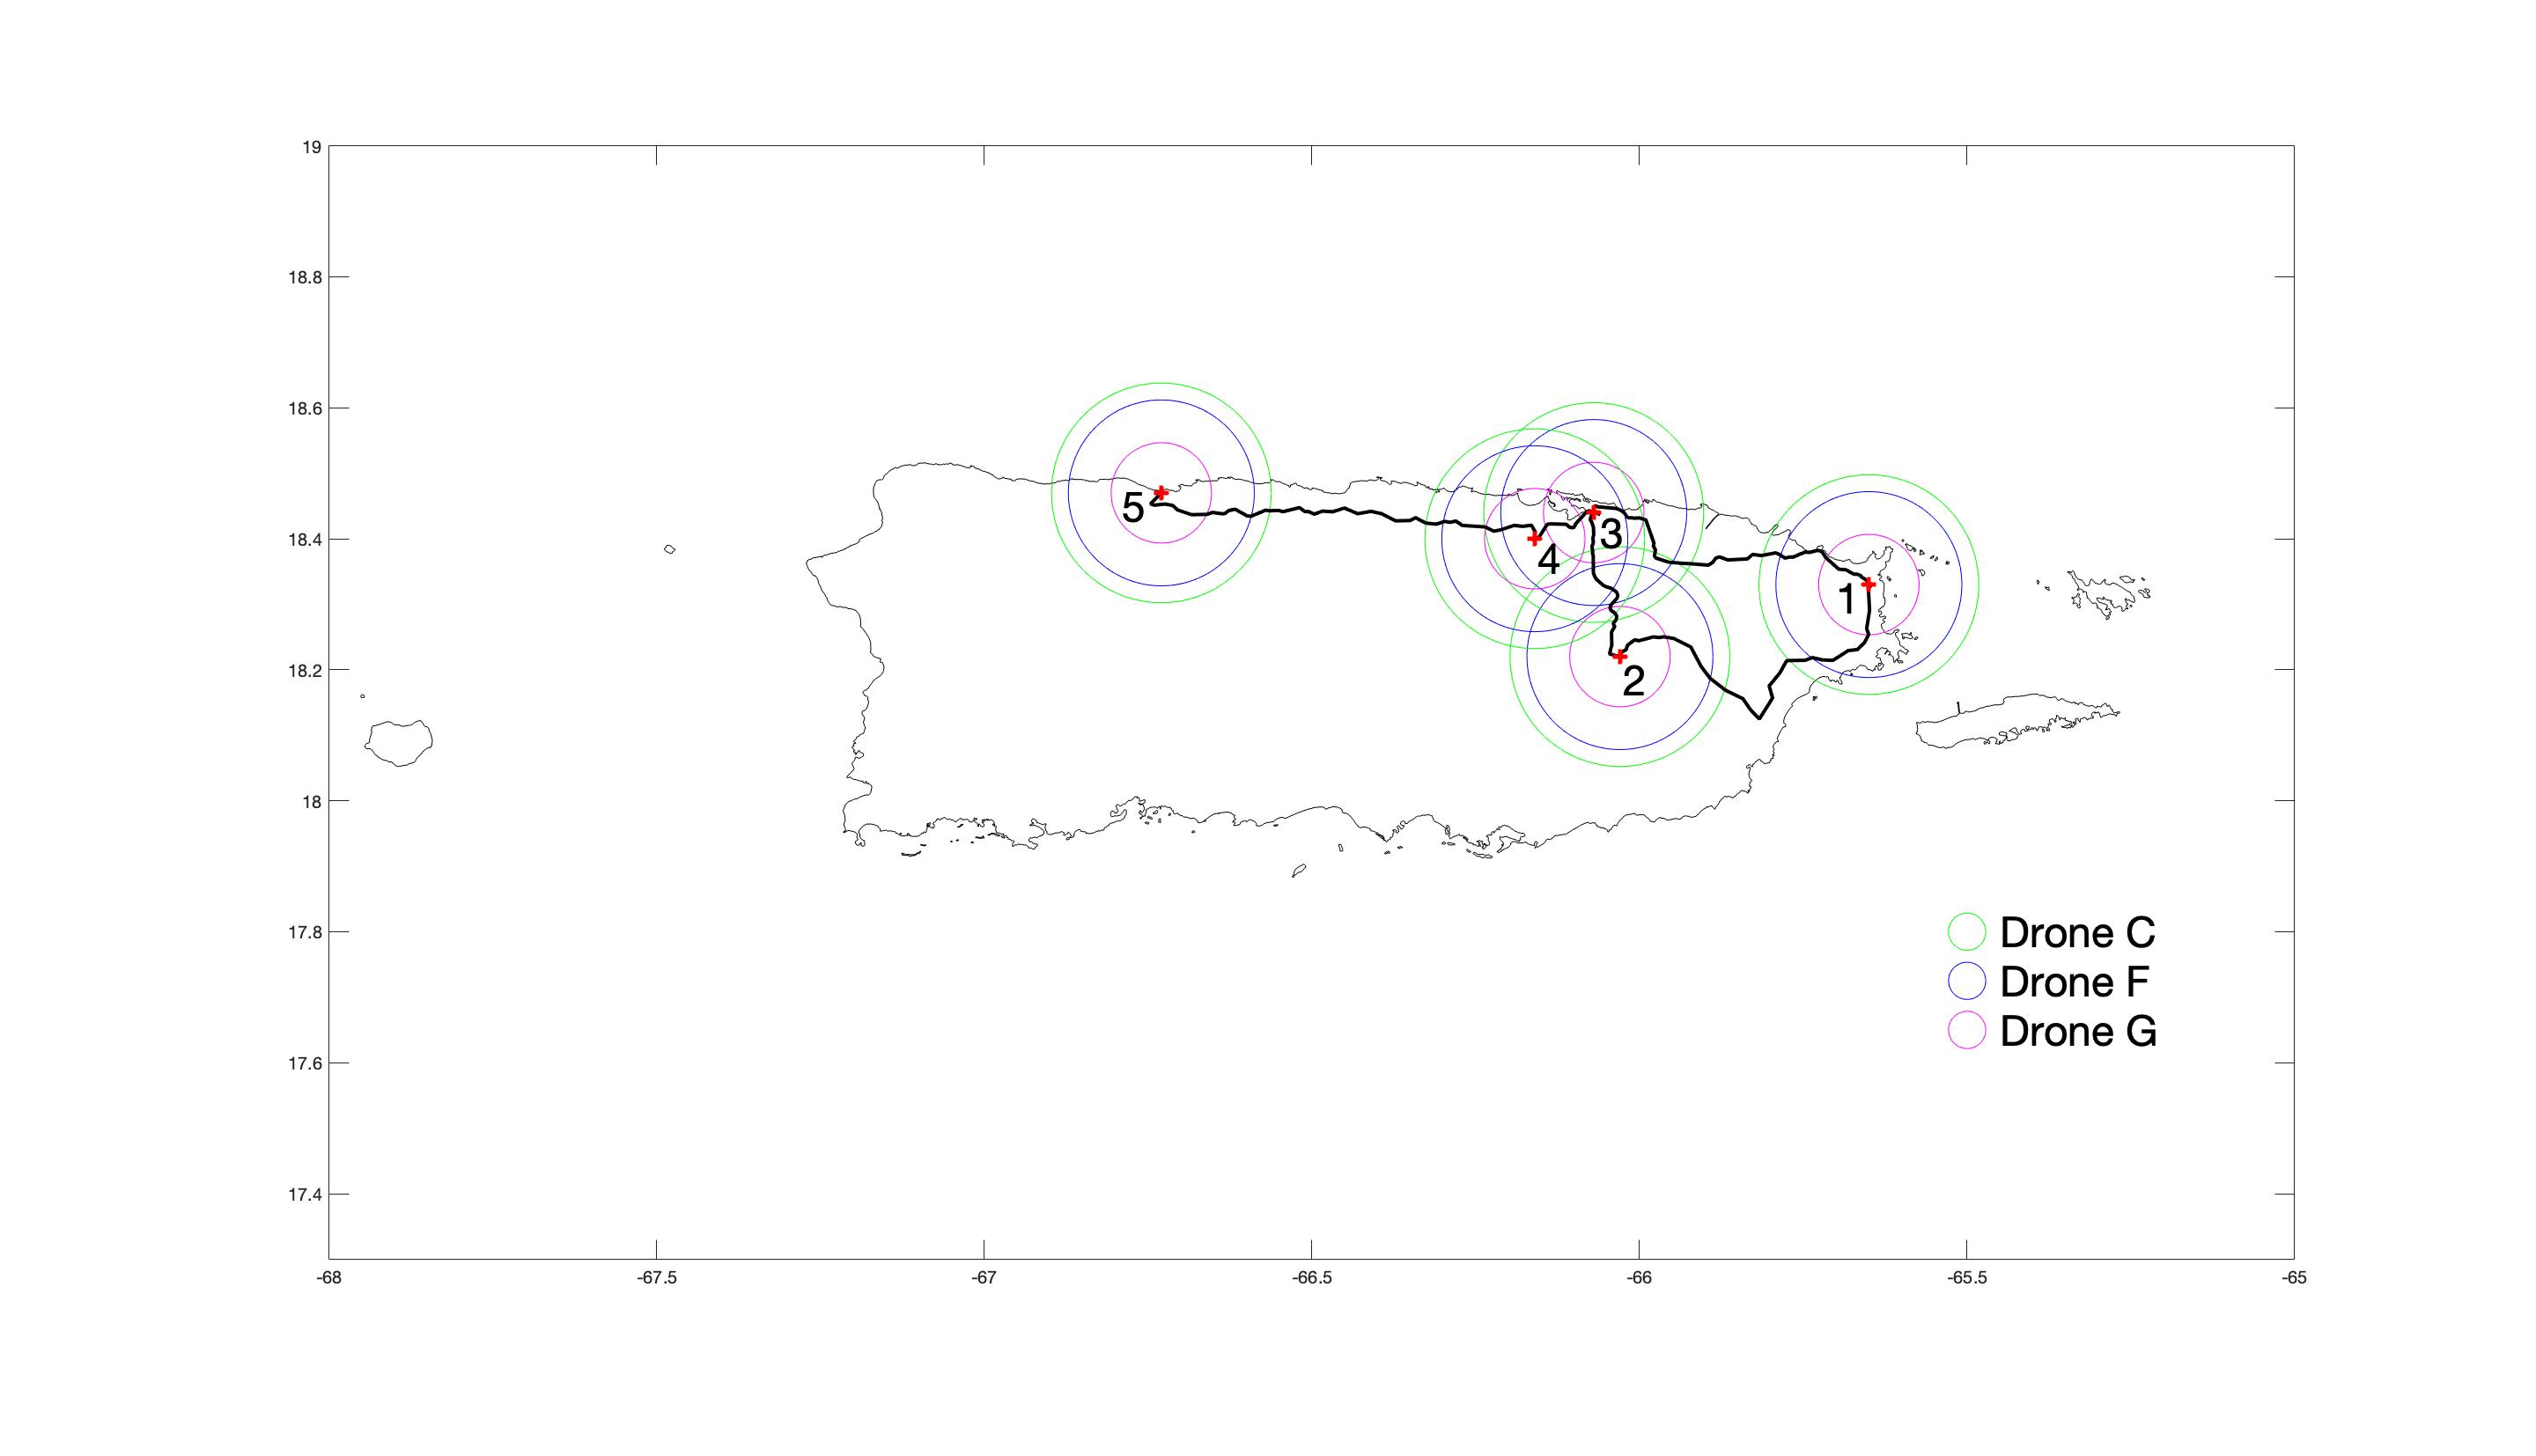
\includegraphics[scale =0.15]{CB2}
\caption{CB2 drone radii around each MC}
\label{cb2}
\end{figure}

\newpage

\subsection{Number of Containers To Use}
Ideally a minimum number of containers should be used to appropriately distribute resources in order to minimize costs.
However looking at the diagrams above we can see that MC1 and MC5 are completely separated from any other MC regardless
of which drone we use$^{*}$. This means that \bf{we must require all three containers} \normalfont{to deliver medical packages to each medical centre.
Since we need three containers we will call them C1, C2 and C3 to save time. Each container will serve the following MCs:}

\begin{center}
\begin{tabular}{ |c|c| }
 \hline
 Container & Medical Centres Served \\\hline
  C1 & MC1 \\
  C2 & MC2, MC3, MC4  \\
  C3 & MC5 \\
 \hline
\end{tabular}
\end{center}

One \bf{key assumption} \normalfont{here is that containers can be placed anywhere we require}. One justification could be that the DroneGo fleet serves as an emergency backup similar to a bomb shelter or food warehouse.
A second justification could be that containers are airdropped in safely.
We can now look at each individual container and determine the packing configuration we want to serve their respective MCs.\\*
\\**
\footnotesize{B can technically service MC1, MC2 and MC3 however, then it wouldn't service MC4}\normalsize{.}

\section{Container Packing Strategy}
In order to solve the problem of packing 3 unique MPs and a drone/s into a container we decided to research bin packing algorithms.
However, we were unable to find an existing algorithm that satisfactorily answered this question with these conditions.
\\*We therefore resorted to developing our own algorithm which we called the \bf{'Cuboid Reduction Method'} \normalfont{that would be able to
efficiently pack different medical packages into the same container.}

\subsection{Cuboid Reduction Method (CRM)}
Our algorithm known as the Cuboid Reduction Method relies on dividing our container into X amount of cuboids with equal dimensions. We then pack each cuboid with only one
type of medical package to avoid the multi-box problem (packing three different boxes into a container).\\* In order to make sure we have the correct balance of each MP we
look at the ratio of the MPs to each other and assign the same ratio of cuboids to each MP.\\*
The INFITTER algorithm from Section 2 is then used to see how many MPs of the same type will fit inside the associated cuboid.
(E.g: A container is split into 10 equally sized cuboids. The associated medical centre requires a 1:1 ratio of MP1 and MP2 packages. Thus we assign 5 cuboids for MP1 and 5 cuboids for MP2.
Note: In the case where cuboids could not be distributed perfectly, the closest ratio was used.
\\*
The CRM was used on C1 and C2 as they both required packing two or three types of MP's. For C3 the INFITTER/OUTFITTER algorithm could be used directly as only one type of MP was being packed.

\subsection{Improving the CRM}
While the cuboid reduction method is useful in assigning a balanced ratio of cuboids for each type of MP, it does have a serious flaw. By assigning the number of cubes that satisfy the MP1 : MP2 : MP3
ratio we ignore the fact that a cube will fit much more MP2s or MP3s than MP1s. This is because they are so much smaller than an MP1.\\*
When running our model initially for C2 and with a required ratio of $5:2:3$  we noticed that our results were giving us quantities of $(1296MP_1, 1620MP_2,990MP_3)$, which go completely against the ratios required for each MP!
In order to solve this we created an algorithm called the RatioCheck algorithm that allocated cuboids to have the closest correct ratios.

\subsubsection{RatioCheck Algorithm}
The RatioCheck algorithm would view the MP1:MP2:MP3 ratio required and find the best balanced ratio of cuboids to satisfy this.

	\begin{algorithm}
	    \caption{MED Pack cuboid Ratio Calculator}
		\begin{algorithmic}[1]
			\Procedure{ratiocalculator}{$cuboidAmt$, $dailyReq$, $cuboidDim$, $medDim$}
			\State $ParameterOne$: The amount of Cuboids available
			\State $ParameterTwo$: The daily requirement of Medical Packages $[MED 1,MED 2,MED 3]$
			\State $ParameterThree$: An array of dimensions of the cuboid
			\State $ParameterFour$: A 2d array of medical package dimensions
			\State $Output$: An array with the required amount of cuboids for each Medical Package
			\State
			\State $ratios \leftarrow [0,0,0]$
			\State $order \leftarrow  [0,0,0]$
			\State
			\State $total \leftarrow 0$
			\For{$i = 1$ to $3$}
			\State $total \leftarrow (total + dailyReq[i])$
			\EndFor
			\State
			\For{$i = 1$ to $3$}
			\State $percentage \leftarrow (dailyReq[i]/total)$
			\State $tempRatio \leftarrow (percentage * cuboidAmt)$
			\State $order[i] \leftarrow (tempRatio - floor(tempRatio))$ \Comment{track the percentage difference}
			\State $ratios[i] \leftarrow floor(tempRatio) $
			\EndFor
			\State
			\State $total \leftarrow 0$
			\For{$i = 1$ to $3$}
			\State $total \leftarrow (total + ratios[i])$
			\EndFor
			\State
			\State $cuboidsLeft \leftarrow (cuboidAmt - total)$
			\State $highestPriority \leftarrow order[i]$
			\State $place \leftarrow 1$
			\For{$i = 2$ to $3$} \Comment{find which med. pack. was most affected by the above process and give it priority}
			\If{$highestPriority< order[i]$}
			\State $highestPriority \leftarrow order[i]$
			\State $place \leftarrow i$
			\EndIf
			\EndFor
			\State
			\State $ratios(place) \leftarrow ratios(place) + cuboidsLeft$ \Comment{dedicate excess cuboid(s) to prioritised}
			\State Return $ratios$
			\EndProcedure
		\end{algorithmic}
	\end{algorithm}

\newpage

\section{Mapping Roads}
In order to balance delivering supplies with performing road reconnaissance we first calculated the maximum packing capabilities of C1, C2 and C3.
Since C1 and C3 only serve MC1 and MC5 they can contain a huge amount of supplies. This led us to deciding to allocate an additional drone to C1, C2 and C3 for purely recon activities.
This way, one drone will deliver the daily MPs to the MC while another drone scans the different roads in the area.\\*\\*
There are a few caveats to this procedure:
\begin{itemize}
\item Firstly, using a drone to scan roads means that extra space must be used in the container to allocate it.
\item Secondly, a drone will travel along approximate straight lines in order to minimize fuel waste. Determining how many straight lines to approximate a road by was done later once the exact coordinates of C1,C2 and C3 were decided.
\end{itemize}

While C1 and C3 could be dropped anywhere within the red circles of Fig 2, since the recon drone is designed to purely assess roads it would be ideal to drop a container on the intersection between the circles circumference and a major road.
This would allow our delivery drone to safely deliver supplies while having the recon drone start immediately on a major highway rather than waste fuel going towards one.

\subsection{Approximating Road Distances}
By using several linear approximations to the roads we could approximate them to measurable quantities. The following map shows the major roads of Puerto Rico, each medical centre as well as approximations for each road.

\begin{figure}[h]
\centering
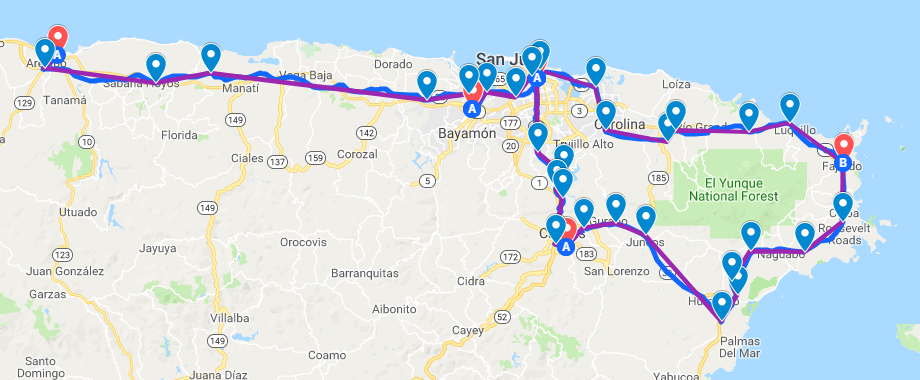
\includegraphics[scale =0.5]{ConnectedLineMap}
\caption{Linear Approximation vs Real Roads}
\label{road-approx}
\end{figure}

\begin{figure}[h]
\centering
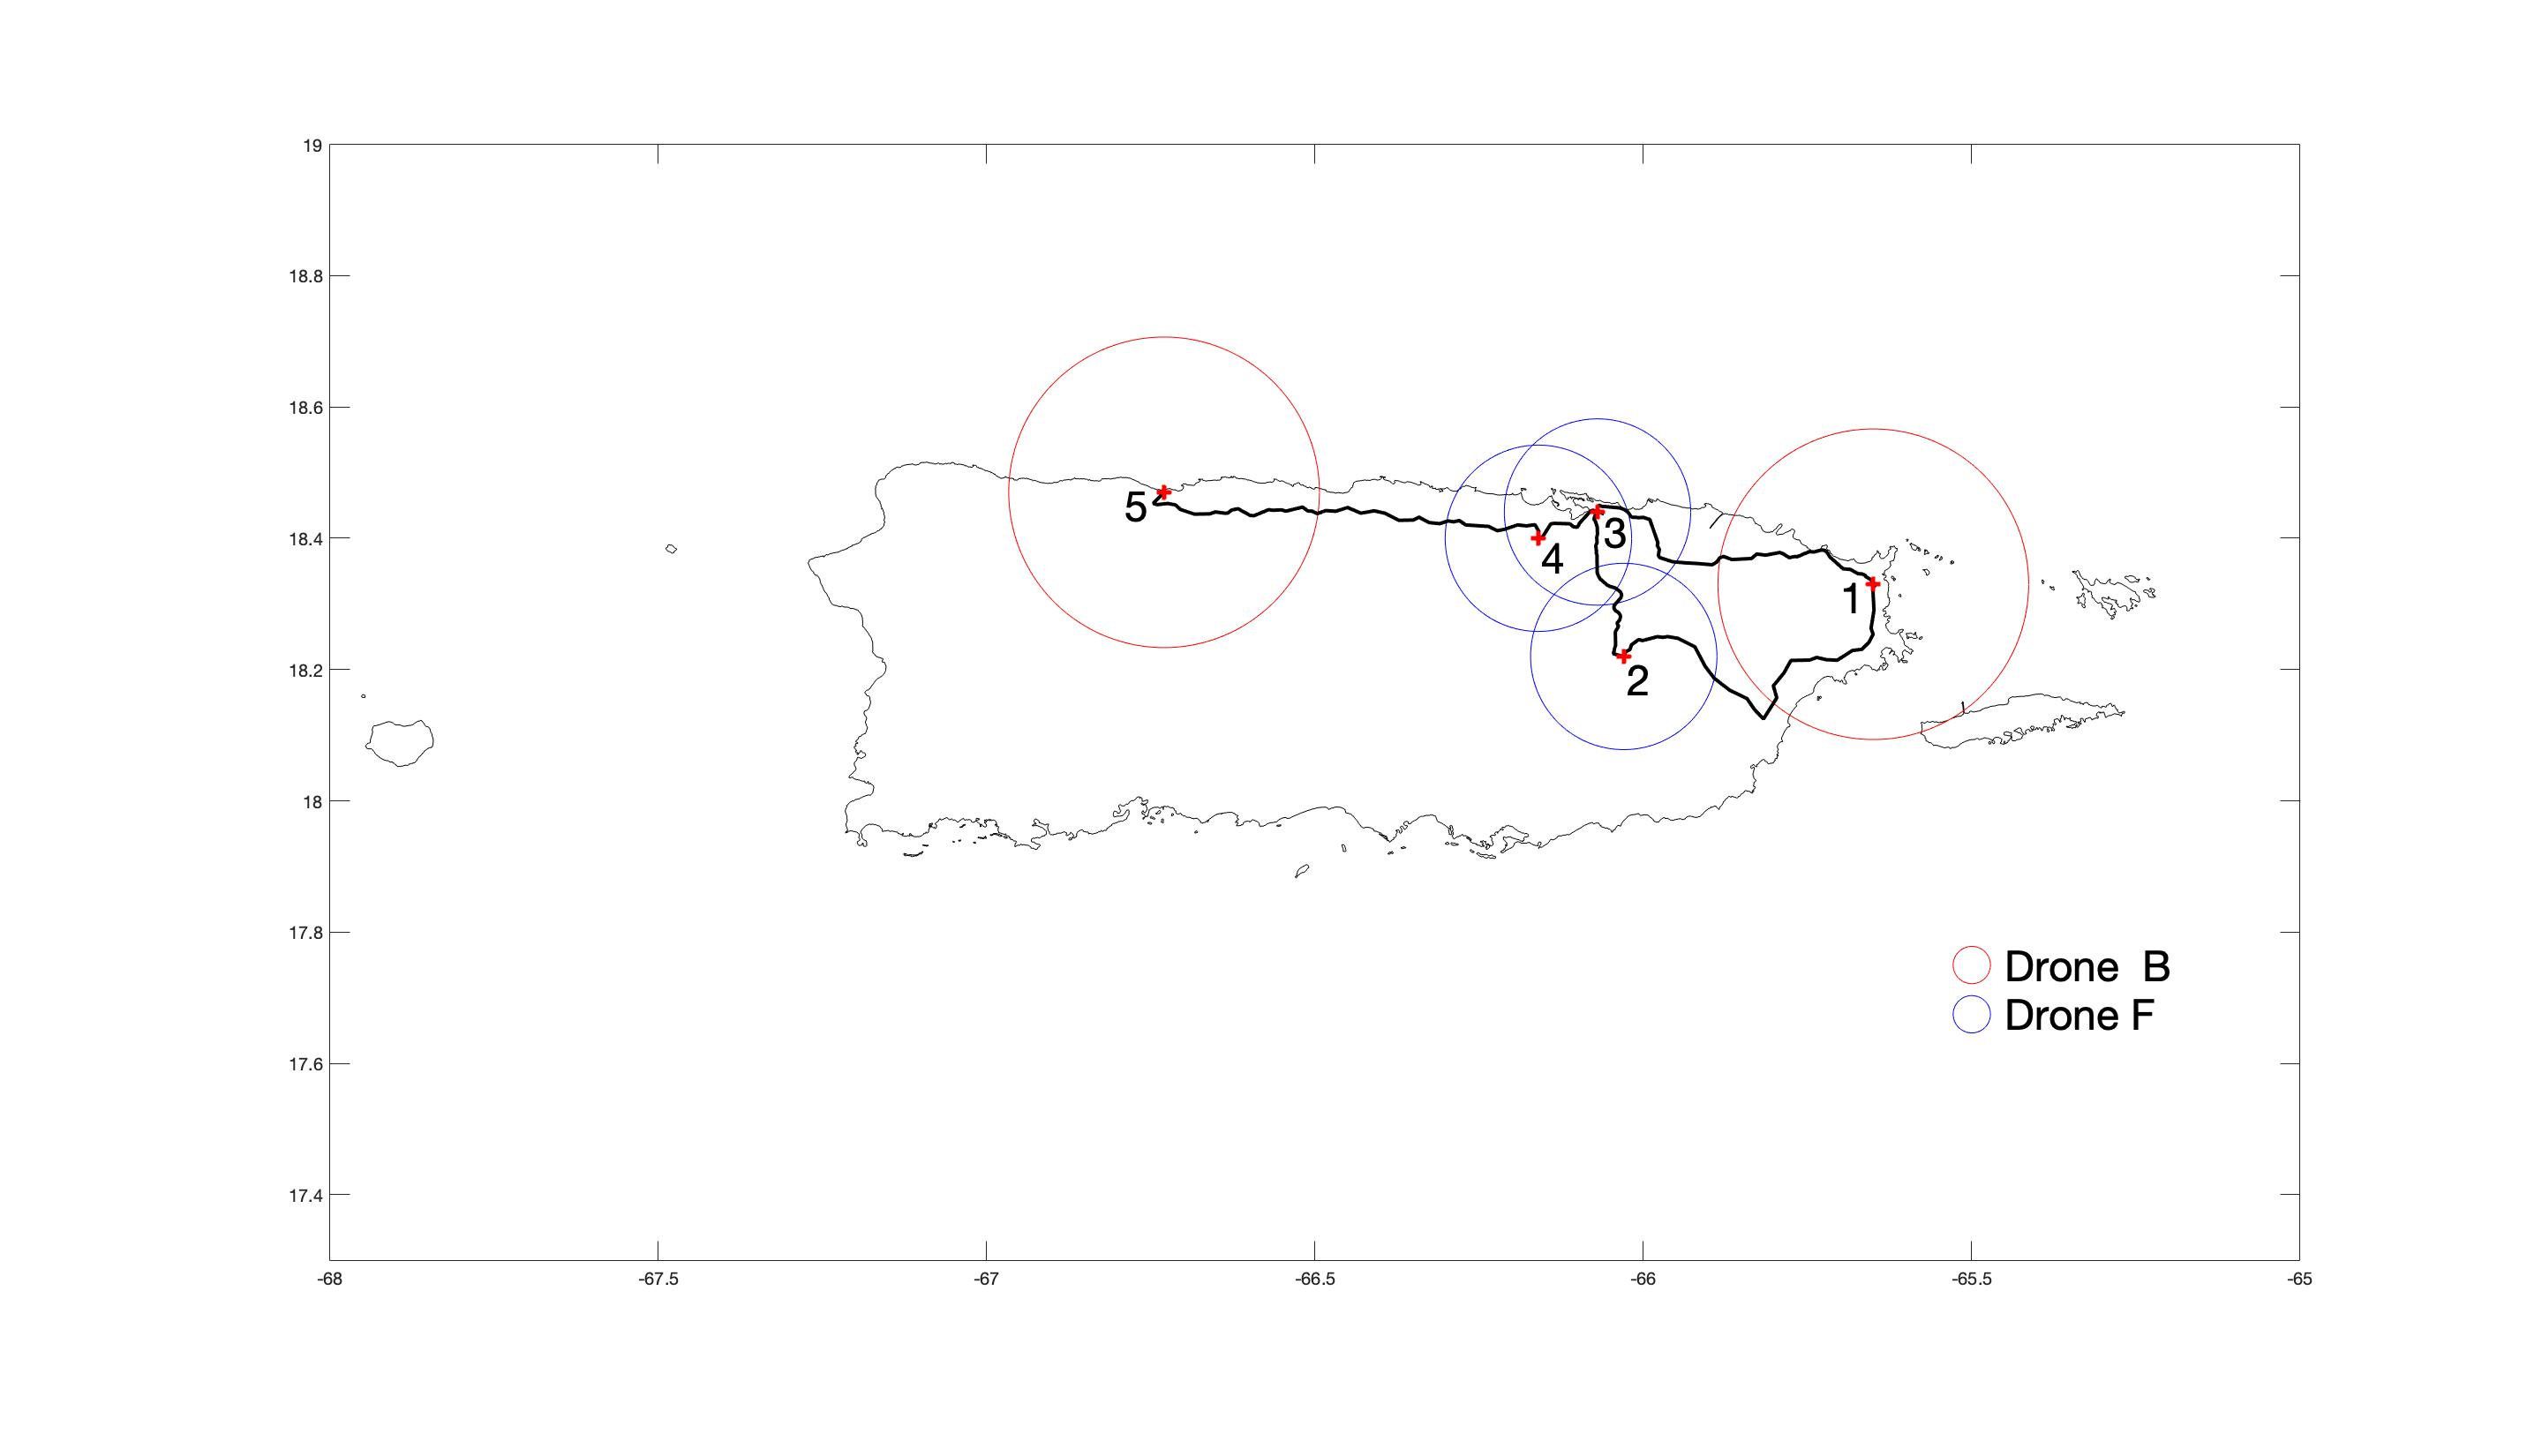
\includegraphics[scale =0.15]{CircleRoadMap}
\caption{Road Map and Delivery Drone Radii}
\label{road-approx}
\end{figure}

\newpage
In Fig 4 the blue lines represent the actual major roads which we wish to follow. The purple line shows our approximated path that we wish the drone to follow. The red pins mark where the hospitals are.\\*
Since the drones will operate at an elevation of 400 feet (121m) we will have a radial field of view of 692 feet (211m). This was based on commercial drones which have a FOV of up to $120^{o}$$.^{8}$
\\*It is a consequence of approximations that there will be times when the road will fall out of the drone's FOV, in order to minimize this error we added more straight lines between roads until the error was negligible.
\\*The following table demonstrates the error percentage between actual road and approximated road total distance.\\*

\begin{center}
\begin{tabular}{ |c|c|c|c|}
 \hline
 Road & Approx Distance (Km) & Actual Distance (Km) & Error Percentage \\\hline
  MC1-MC2 & 66.5 & 68 & 2.21\% \\
  MC1-MC3 & 58 & 58.1 & 0.17\% \\
  MC2-MC3 & 31.7 & 32 & 0.94\%  \\
  MC3-MC4 & 13.4 & 13 & 3.04\% \\
  MC4-MC5 & 70.1 & 71 & 1.27\%  \\
 \hline
\end{tabular}
\end{center}

We could also argue that heavy road damage will be visible for large stretches of the road so we could predict if unseen segments are damaged based on previous parts of the road.

\newpage

In Fig 5 we further approximate our roads and place them into our generated map of Puerto Rico with the radial circles that correspond to the specific drone range of each MC.
This way we will place our containers right on the intersection of the delivery drone radius with the major roads.  While we have some leeway on choosing container coordinates for C2 and C3 we decided to pick the following coordinates:

\begin{center}
\begin{tabular}{ |c|c| }
 \hline
 Container & Container Coordinates (Long and Lat) \\\hline
  C1 & -65.88 18.37 \\
  C2 & -66.04 18.32  \\
  C3 & -66.5 18.44  \\
 \hline
\end{tabular}
\end{center}

\newpage

\subsection{Road Recon Model (RRM)}
Our Road Recon Model was designed in order to maximize reconnaissance range i.e. to map as much road length as possible.
With our container coordinates, we decided to use drone B for recon as it has the furthest range of 24.4 km.
Plotting the distance along each road from our container coordinate we were able to obtain the following map. This gives us a clear view of how far
a recon drone would be able to travel down any road and back.

\begin{figure}[h]
\centering
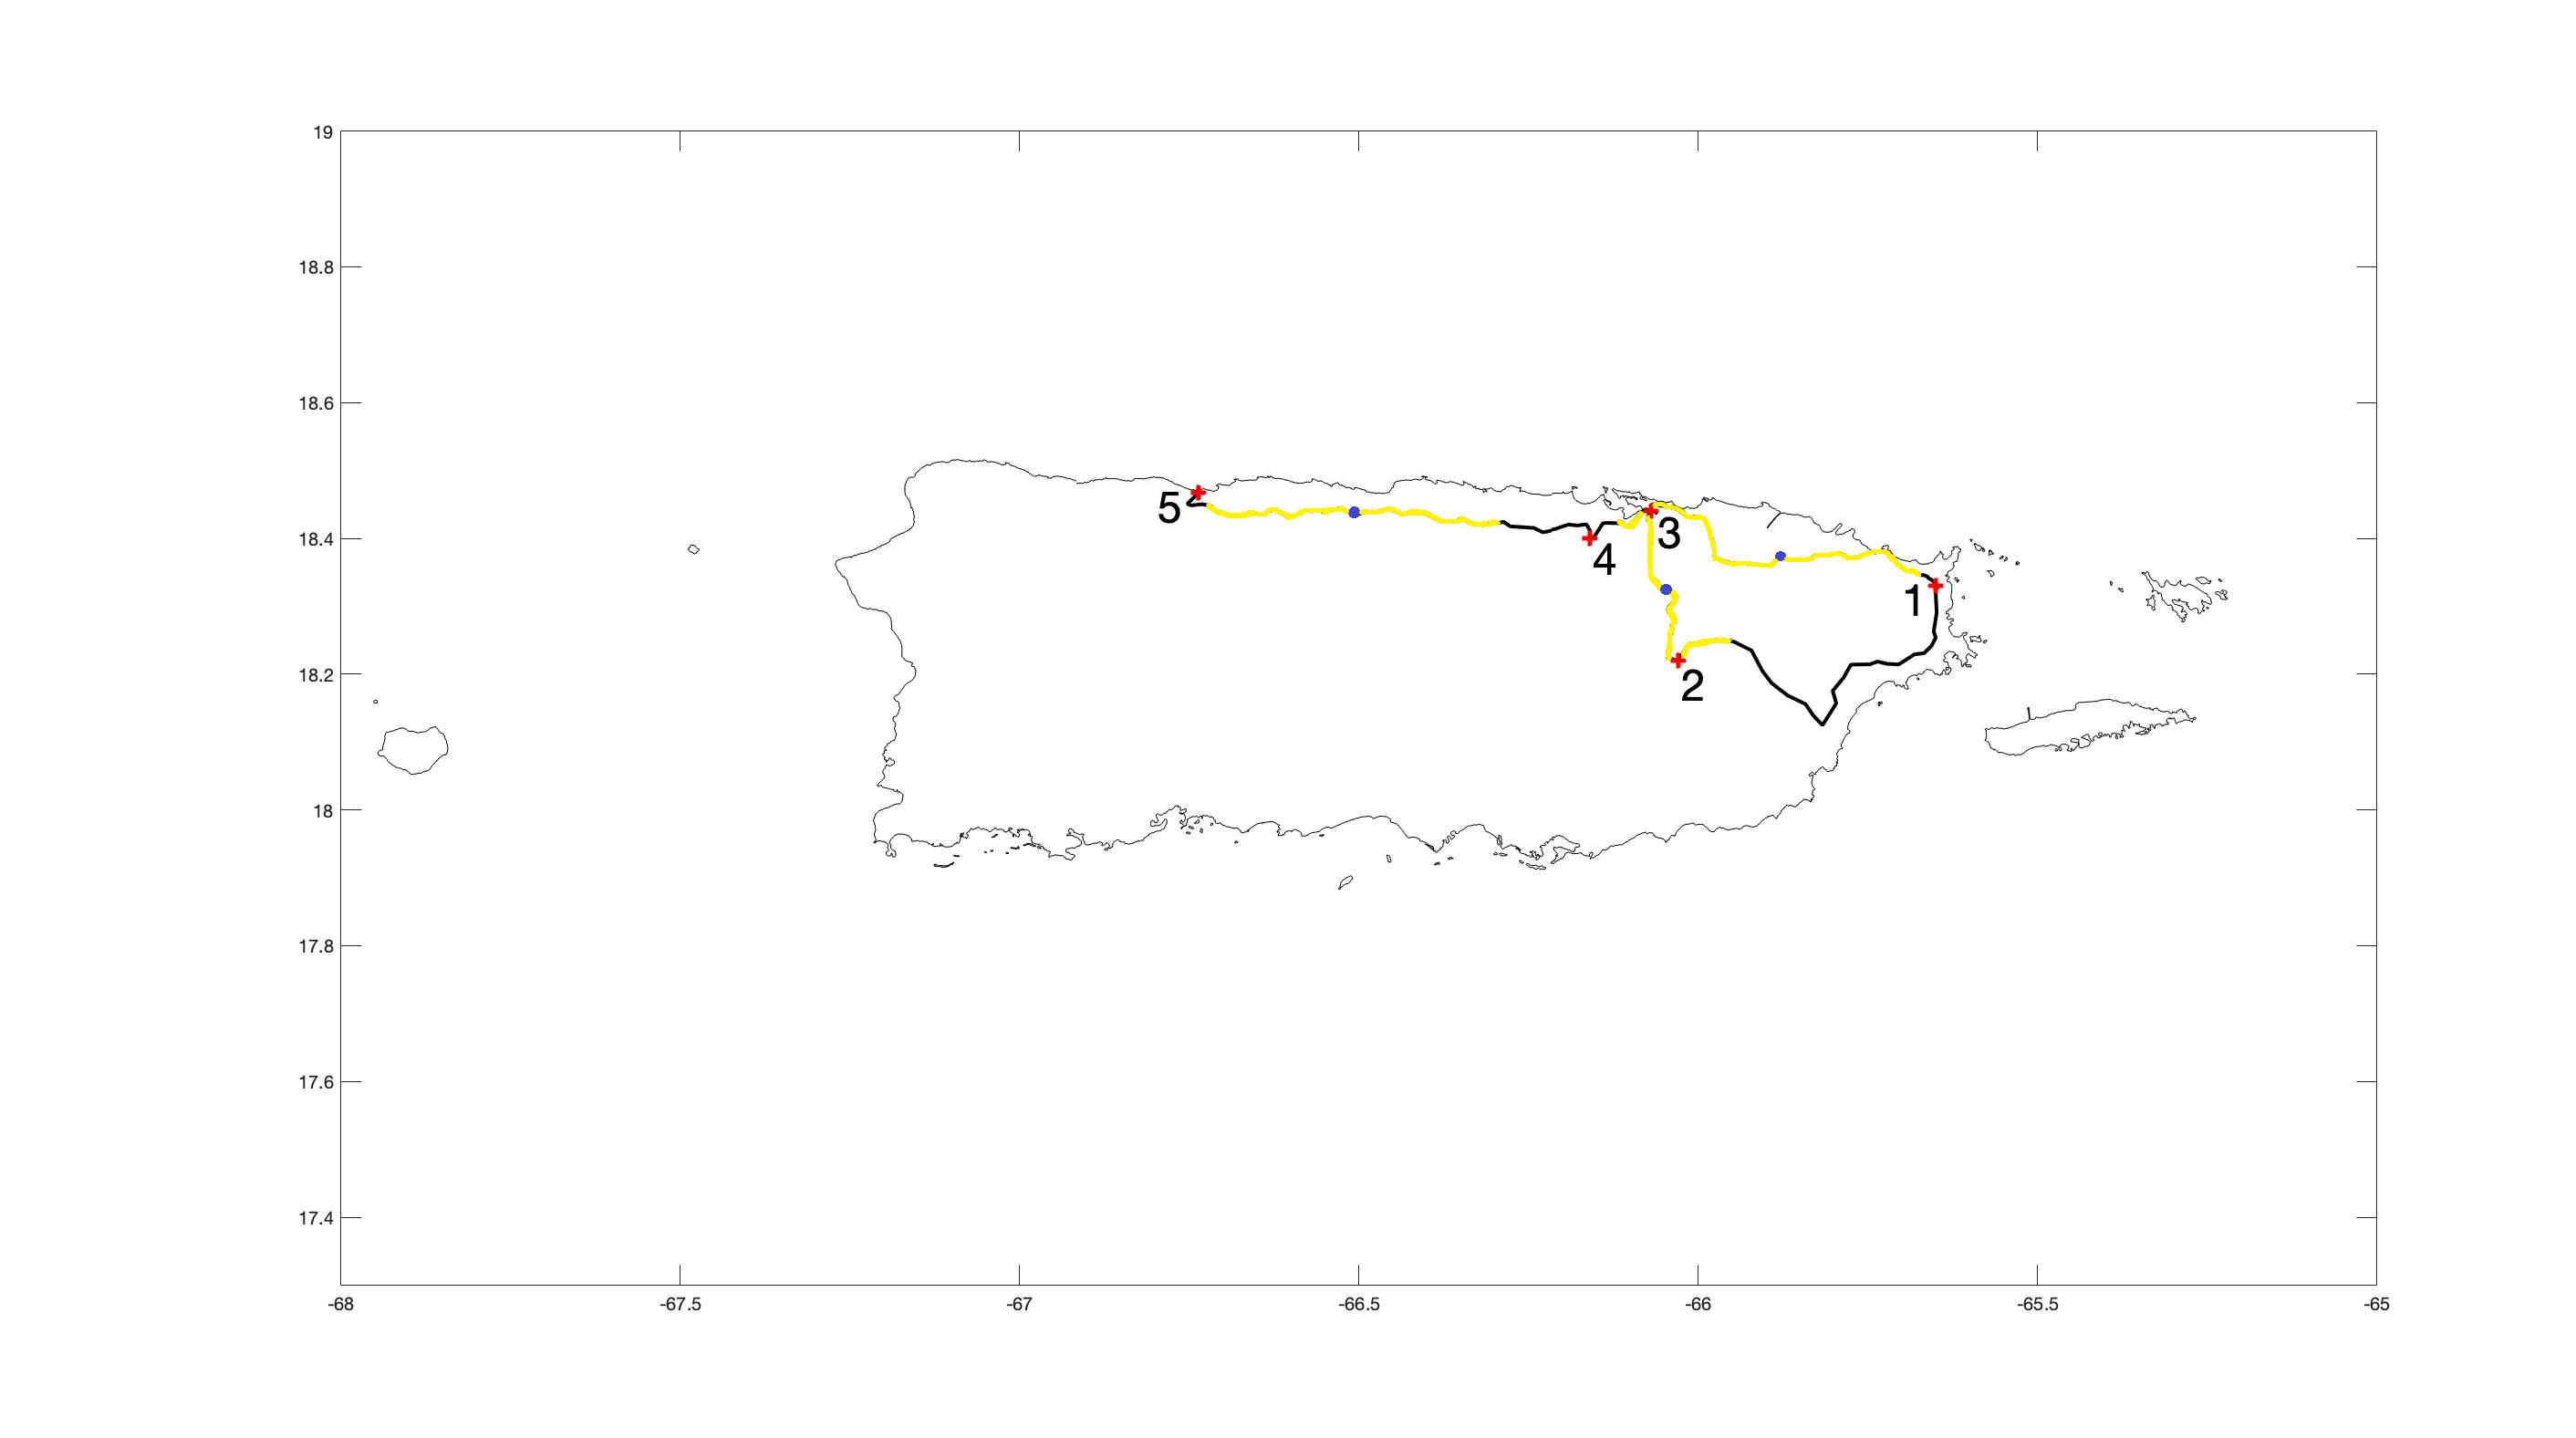
\includegraphics[scale =0.18]{NewRoadNoCircles}
\caption{Road Map}
\label{road-approx}
\end{figure}

The yellow lines represent the distance a recon drone will travel from the container location which is marked blue. Looking at this we can immediately see that the major roads
between MC1, MC2, MC3 and MC4 are (almost) completely covered except for small region beside MC1.
Likewise the yellow region from C3 to MC5 almost completely reaches MC5 but stops just short. This is still a very large region of road that the drones can scan
and demonstrates the power of aerial surveillance that they can achieve for ground based route planning.


\newpage

\section{Applying Model to 2017 Crisis}
Benchmarking is an important step in testing any product or service and this is no different from our model. By comparing our approach with the actual approach used we can see if our model holds any actual value in assisting
in the delivery of supplies to centres.

\subsection{2017 Crisis Official Figures}
When Hurricane Maria struck Puerto Rico the entire island's electrical grid was wiped out. It took 7 months before electricity was restored to 97.7 %
of the population.$^8$ Using this figure we can test our model to see if we can provide supplies to the medical centres for up to and (if necessary) over 7 months.
Road damage to Puerto Rico during the hurricane was also extensive but figures are much harder to find due to the slow progress of repairs. We will assume that road repairs will take at
least 7 months if not more.

Major highways in Puerto Rico were damaged as well during the disaster.

\subsection{Strategy 1}
Our first and simplest strategy of utilizing our model to deal with the 2017 Puerto Rico crisis was as follows;

\begin{itemize}
\item[-]Drop or have all three containers at their respective locations as specified in (7.1)
\item[-]Implement the RRM and CRM to scanning roads and packing supplies for each container
\end{itemize}

\subsubsection{Drone Package Configuration and Schedule}

The following configurations were tabulated for each medical centre.



Container 1\\*\\*
\begin{tabular}{ |c|c|c| }
 \hline
 Drone & Payload & Route \\\hline
  F & $MP_1,MP_3$ & MC1 \\
  B & NA & RECON \\
 \hline
\end{tabular}

Container 2\\*\\*
\begin{tabular}{ |c|c|c| }
 \hline
 Drone & Payload & Route \\\hline
  F & $MP_1,MP_1,MP_3$ & MC2 \\
  F & $MP_1,MP_2$ & MC3   \\
  F &  $MP_1,MP_1,MP_2,MP_3,MP_3$ & MC4 \\
  B & NA & RECON \\
 \hline
\end{tabular}

Container 3\\*\\*
\begin{tabular}{ |c|c|c| }
 \hline
 Drone & Payload & Route \\\hline
  F & $MP_1$ & MC5 \\
  B & NA & RECON \\
 \hline
\end{tabular}

\subsubsection{Results}
We obtained the following data for how long supplies would last for each container area:

\begin{center}
\begin{tabular}{ |c|c|c|c| }
 \hline
  & C1 & C2 & C3 \\\hline
  $MP_1$ & 1458 & 1458 & 2916 \\
  $MP_2$ & 0 & 1215 & 0  \\
  $MP_3$ & 1782 & 792 & 0 \\
  Recon Drone & B & B & B \\
  Delivery Drone & B & 3F & B \\
  Days & 1558 (4.2 years) & 264 (8.6 months) & 2916 (7.9 years) \\
 \hline
\end{tabular}
\end{center}

As we can see this strategy successfully provides medical packages for each medical centre for months or even years. Since 7 months is the time it took
This strategy also allows us to cover 60%

\subsection{Optimizing this Strategy}
In this alternative strategy we consider using the fact that C1 and C3 will last much longer than C2 by several years.
We also consider the fact that the maximum range of a drone is twice the normal range of a drone that returns back to a container.
Using these facts we came up with the idea of fitting an two extra Recon drones to both C1 and C3. This drone's purpose would be to travel as far as possible
in order to scan the most road possible without returning.\\*
We calculated that with this strategy we could cover 100% of the road network between all the medical centres while only losing ~400 days for C1 and ~300 days for C3.
Considering that this still means C1 and C3 can last years more than C1 we concluded this was worthwhile.

The only drawback to this is that an expensive drone has been lost somewhere down the road but this is small in light of the cost of repairs.



\newpage

\section{Conclusions}
To conclude our model allowed us to deal with the Puerto Rico crisis to a very satisfactory degree. We were able to map 100\% of the major road network between each medical centre and provide supplies that would last
months or even years. Medical centre 1 and 5 were able to be supplied for years and the others could last just more than 8 months.
One drawback with our CRM was that we did not implement existing bin packing algorithms that would have surely given us the optimal packing. However the optimal packing was not necessary due to the fact that all 3 containers were used.
Using all three containers was completely necessary due to the distance between medical centres. \\*
With further time we would have researched and tried to discover more optimal bin packing algorithms as well as strategies for placing containers regardless of where the medical
centres were located. The CRM could have also been improved by designing the ratio calculator to be more efficient in distributing packages.


\newpage

\section{References}

\begin{enumerate}
\item CIA. 2019. Central America :: Puerto Rico — The World Factbook. [ONLINE] Available at: https://www.cia.gov/library/publications/the-world-factbook/geos/rq.html. [Accessed 26 January 2019]
\item USGS. 2016. USGS CFWSC - Climate of Puerto Rico. [ONLINE] Available at: https://pr.water.usgs.gov/drought/climate.html. [Accessed 26 January 2019]
\item Ezcurra, Rivera-Collazo. 2017. An assessment of the impacts of climate change on Puerto Rico's Cultural Heritage with a case study on sea-level rise. [ONLINE] \\*Available at: https://www.sciencedirect.com/science/article/pii/S1296207417306441. [Accessed 26 January 2019]
\item FEMA. 2019. Hurricane Maria | FEMA.gov. [ONLINE] Available at: https://www.fema.gov/hurricane-maria. [Accessed 27 January 2019].
\item Nikos Drakos. 1996. Bin Packing. [ONLINE] \\*Available at: https://www8.cs.umu.se/kurser/TDBA77/VT06/algorithms/\\*BOOK/BOOK5/NODE192.HTM. [Accessed 26 January 2019]
\item Brian Schneider. 2018. A Guide to Understanding LiPo Batteries. [ONLINE] Available at: https://rogershobbycenter.com/lipoguide/. [Accessed 26 January 2019]
\item FAA. 2019. eCFR; Code of Federal Regulations. [ONLINE] Available at: https://www.ecfr.gov/cgi-bin/text-idx?SID=dc908fb739912b0e6dcb7d7d88cfe6a7\&mc\\*=true\&node=pt14.2.107\&rgn=div5. [Accessed 27 January 2019]
\item Softonic. 2018. ProMark Camera Drone B07B9 - Get Now. [ONLINE] Available at: https://en.softonic.com/solutions/electronics/promark-camera-drone-b07b9. [Accessed 26 January 2019]
\item FAA. 2019. eCFR; Code of Federal Regulations. [ONLINE] Available at: https://www.ecfr.gov/cgi-bin/text-idx?SID=dc908fb739912b0e6dcb7d7d88cfe6a7\&mc\\*=true\&node=pt14.2.107\&rgn=div5. [Accessed 27 January 2019]
\end{enumerate}

\newpage

\section{Appendix}
Here is extra pseudo-code for the CRM for the interested reader.

\begin{algorithm}
  \caption{Cuboid Reduction Method}
\begin{algorithmic}[1]
  \Procedure{crm}{$droneAmount$, $dailyRequiremnt$}
  \State $ParameterOne$: The amount of drones needed for the container
  \State $ParameterTwo$: The daily requirement of Medical Packages $[MED 1,MED 2,MED 3]$
  \State $Output$: The amount of days a container of supplies can last
  \State
  \State $cuboid \leftarrow [46, 46, 47]$
  \Comment{The dimensions of our cuboid}
  \State $medPs \leftarrow  [14, 7, 5 ; 5, 8, 5 ; 12, 7, 4]$ \Comment{2d Array of Medical Package Dimensions}
  \State $cuboidsLeft \leftarrow 20 - droneAmount$ \Comment{Amount of cuboids left after we pack in drones}
  \State
  \State $packRatios \leftarrow RATIOCALCULATOR(cuboidsLeft, dailyRequirment, cuboid, medPs)$
  \State
  \State $packAmount \leftarrow [0,0,0] $
  \For {$i = 1$ to $3$ }
  \State $packAmount[i] \leftarrow ( INFITTER(cuboid, medPs[i] ) * packRatios[i] )$
  \EndFor
  \State
  \State Return $DAYCALCULATOR(dailyRequirement, packAmount)$
  \EndProcedure
\end{algorithmic}
\end{algorithm}

\end{document}
